\newpage
\section{Überblick über den strukturellen Aufbau und Inhalt des Dash\-boards}
\label{ch:Dashboard:sec:Aufbau}


Die Daten aus den Oberflächen des alten Systems werden auf zwei Dash\-boards aufgeteilt. Dabei gibt es je eins für die Entwicklungsversion und eins für alle veröffentlichten und aktiv gewarteten Versionen (Release-Versionen). Da die Release-Versionen bis auf kleinere Fixes kein Bestand des Tagesgeschäfts mehr sind, ist die Anzahl der benötigten Tests bedeutend geringer. Somit kann der Statusbericht mehrerer Versionen gesammelt auf einem seperaten Dash\-board angezeigt werden.

Grafana gibt eine Dash\-board"=Struktur in Reihen vor. Jede Reihe stellt ein System dar, welches im alten System jeweils eine eigene Seite benötigt. Diese Reihen sind für die Übersichtlichkeit zusätzlich einklappbar. Die Panele einer Reihe sind in drei Spalten aufgeteilt (s. \autoref{fig:aufbau_dashboard}).

\begin{figure}[H]
    \centering
    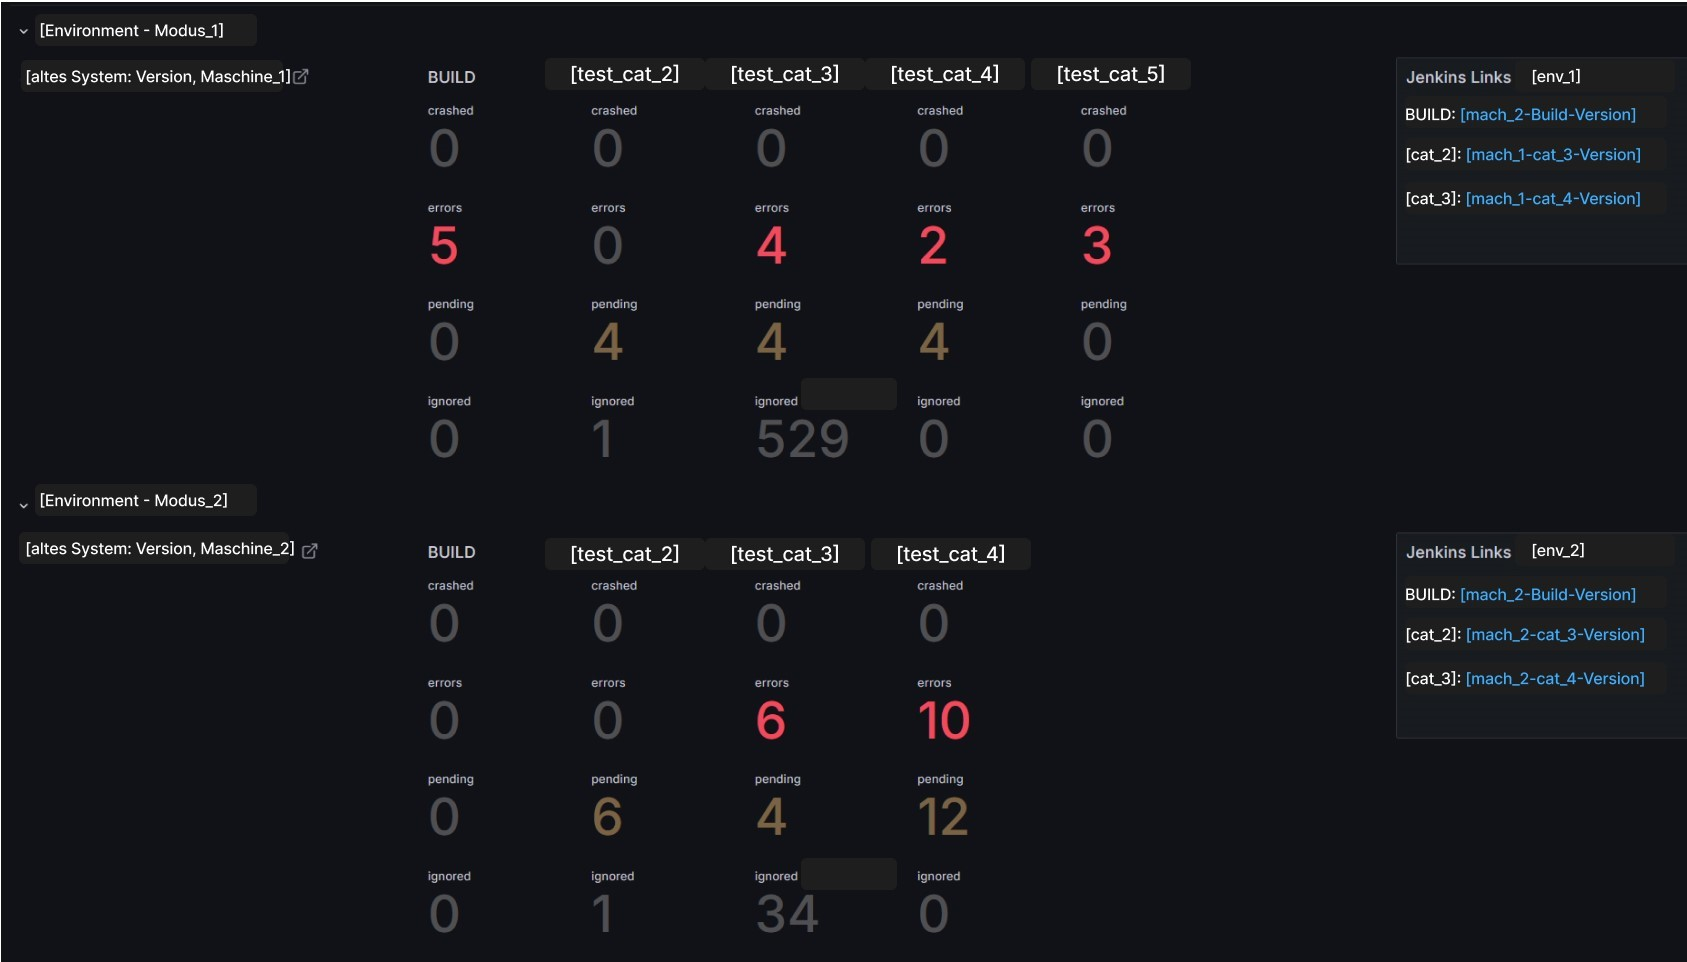
\includegraphics[width=1\linewidth]{Dashboard/Dashboard_zensiert.jpg}
    \caption{Aufbau des entwickelten Dashboards}
    \label{fig:aufbau_dashboard}
\end{figure}

% mittlere Spalte
\noindent
Die jeweilige Fehlerzahl bzw. der Zustand der entsprechenden Testkategorie wird in der mittleren Spalte in verschiedenen Farben dargestellt.
Im Falle eines Green Days, ein Tag an dem keine Fehler auftreten, steht in allen Feldern eine dunkelgraue Null. Um die Relevanz des Fehlerfalls darzustellen, werden diese Zahlen farbig hervorgehoben (s. \autoref{ch:SdF:UI:sec:menschenzentriertes_Design}). Die Fehlerkategorien sind 'System abgestürzt', 'Anzahl der Fehler', 'Anzahl der ausstehenden Tests' und 'ignorierte Tests'\footnote{Die Kategorie 'Ignorierte Tests' umfasst zum Beispiel Testfälle mit länger bekannten Fehlern, die für die Einschätzung des Green Days ignoriert werden dürfen.}.
Aufgrund der Menge an Testfällen und der Anforderung, alle zusammengehörigen Daten auf einen Blick erfassen zu können (s. \autoref{ch:Dashboard:sec:Anforderungen}), sind die Test-Kategorien in Spalten und deren Ergebnisse in den Reihen darunter dargestellt. Im Vergleich zum alten System wurden die Reihen und Spalten vertauscht (s. \autoref{fig:aufbau_altes_System}).

% Informationen: linke + rechte Spalte
Neben den System-Zustandsinformationen, die auch das alte System anzeigt, bietet das Dash\-board die Gelegenheit, weitere Informationen zu sammeln und zur Verfügung zu stellen.
Links ist unter dem Reihentitel die Verlinkung auf die Oberfläche des alten Systems zu finden. Dieses bietet genauere Informationen im Fehlerfall (s. \autoref{ch:IST-Zustand:sec:Aufbau_altes_System}).
Für detailliertere Informationen zu den Fehlern werden die Jenkins-Jobs der einzelnen Testkategorien in der Spalte auf der rechten Seite aufgelistet.

In der nachfolgenden \autoref{tab:Funktions_Mapping:alt_auf_neu} werden die Unterschiede in Funktionen und Eigenschaften beider Systeme noch einmal gegenübergestellt.

\begin{table}[H]
    \begin{adjustbox}{width=\textwidth}
    \begin{tabular}{|l|c|lc|}
    \hline
                                                                                                         & \multicolumn{1}{l|}{altes System}                                                                                                                                                                                                                                  & \multicolumn{2}{l|}{Dashboard}                                                                                                                                                     \\ \hline
    \begin{tabular}[c]{@{}l@{}}Für den täglichen Monitoring-\\ Prozess benötigt\end{tabular}             & bis zu 30 Oberflächen                                                                                                                                                                                                                                              & \multicolumn{2}{c|}{2 Dashboards}                                                                                                                                                  \\ \hline
    \begin{tabular}[c]{@{}l@{}}Übersicht eines System,\\ einer Maschine \& Version\end{tabular}           & eine Oberfläche                                                                                                                                                                                                                                                    & \multicolumn{2}{c|}{eine Reihe der selben Oberfläche}                                                                                                                              \\ \hline
    \multirow{3}{*}{Inhalt einer Oberfläche}                                                             & \multicolumn{1}{l|}{\multirow{3}{*}{\begin{tabular}[c]{@{}l@{}}Übersicht eines Systems, einer\\ Maschine \& Version\\ $\rightarrow$ eine Testkategorie je Reihe\end{tabular}}}                                                                                     & \multicolumn{2}{c|}{eine Testkategorie je Spalte}                                                                                                                                  \\ \cline{3-4} 
                                                                                                         & \multicolumn{1}{l|}{}                                                                                                                                                                                                                                              & \multicolumn{1}{l|}{Develop}         & \begin{tabular}[c]{@{}c@{}}alle benötigten Kombi-\\ nationen aus System,\\ Maschine \& Version\\ in jeweils einer Reihe\end{tabular}        \\ \cline{3-4} 
                                                                                                         & \multicolumn{1}{l|}{}                                                                                                                                                                                                                                              & \multicolumn{1}{l|}{Release}         & beide Release-Versionen                                                                                                                     \\ \hline
    \multirow{2}{*}{Angezeigte Ergebnisse}                                                               & \begin{tabular}[c]{@{}c@{}}je Testsammlung (ca. 20-80 pro\\ Oberfläche) wird ein Fehlerstatus\\ angezeigt\end{tabular}                                                                                                                                             & \multicolumn{2}{l|}{\begin{tabular}[c]{@{}l@{}}zusammengefasste Zahlen-Werte\\ pro Fehlerkategorie / -status\end{tabular}}                                                         \\ \cline{2-4} 
                                                                                                         & \begin{tabular}[c]{@{}c@{}}Fehler können abhängig von\\ der Testkategorie als Status (\textit{Err},\\ \textit{OK}, \textit{-}, \textit{CORE}) oder als Fehler-\\ anzahl dargestellt werden.\end{tabular}                                                                                               & \multicolumn{2}{l|}{\begin{tabular}[c]{@{}l@{}}Anzahl der jeweiligen Stati (\textit{crashed},\\ \textit{errors}, \textit{pending}, \textit{ignored})\\ $\rightarrow$ jede Kategorie hat dasselbe Layout\end{tabular}} \\ \hline
    Anzeige des Green Days                                                                               & \multicolumn{1}{l|}{\begin{tabular}[c]{@{}l@{}}ausschließlich: \textit{Null} oder \textit{OK}\\ $\rightarrow$ keine roten Hervorhebungen\\       oder andere Zahlen\\ $\rightarrow$ Hintergrundwissen benötigt,\\       welche Werte ignoriert\\       werden dürfen\end{tabular}} & \multicolumn{2}{l|}{\begin{tabular}[c]{@{}l@{}}ausschließlich dunkelgraue \textit{Null}\\ $\rightarrow$ keine roten Zahlen\end{tabular}}                                                   \\ \hline
    \multirow{2}{*}{\begin{tabular}[c]{@{}l@{}}Zugang zu weiterführenden\\Informationen\end{tabular}} & \multirow{2}{*}{\begin{tabular}[c]{@{}c@{}}Verlinkung jedes Testcases\\ hinter dem Testnamen führt zur\\ Terminalausgabe des Testverlaufs\end{tabular}}                                                                                                            & \multicolumn{2}{c|}{\begin{tabular}[c]{@{}c@{}}Verlinkung zum alten System\\ direkt unter der Reihenbeschreibung\end{tabular}}                                                     \\ \cline{3-4} 
                                                                                                         &                                                                                                                                                                                                                                                                    & \multicolumn{2}{c|}{\begin{tabular}[c]{@{}c@{}}Verlinkung zu den einzelnen Jenkins-\\ Jobs aufgelistet nach Kategorie-\\ namen\end{tabular}}                                       \\ \hline
    \end{tabular}
    \end{adjustbox}
    \caption{Überblick und Zuordnung der alten Funktionalität und Arbeitsweise auf das neue Dash\-board}
    \label{tab:Funktions_Mapping:alt_auf_neu}
\end{table}